\documentclass[journal]{IEEEtran}

\usepackage{float}
\usepackage{amsmath}
\usepackage{amssymb}
\usepackage{graphicx}
\usepackage{subfig}
\usepackage{epstopdf}
\usepackage{enumitem}
\usepackage{tikz}
\usetikzlibrary{arrows,automata}
\usepackage{pgfplots}
%\usepackage{tikz,times}

\begin{document}

\section{New correlation coefficient}
\subsection{definition}
    Let$(x_{i},y_{i}),i=1,\dots ,N$,be two time series of length N.Rearranging the two time series with respect to the magnitudes of $x$ and $y$ respectively,we get two new time series denoted by $(x_{(i)},y_{(i)})$,where $x_{(1)}\leq \dots \leq x_{(N)},y_{(1)}\leq \dots \leq y_{(N)}$ are called the \emph{order statistics } of $x$ and $y$. If the Pearson's coefficient $r_{P}(x,y)\geq 0$ ,we define the new correlation coefficient, as follows: \begin{equation} \label{equ:def1}
    r_{N}(x,y)\overset{\bigtriangleup }{=}\frac{r_{P}(x,y)}{r_{P}(x_{(i)},y_{(i)})}.
    \end{equation}

    If $r_{P}(x,y)<0$,let $z_{i}=-x_{i}$.Rearranging the new time series $z_{i}$ with respect to the magnitudes of $z$,we get new series denoted by $z_{(i)}$.We define the new correlation coefficient,as follows:
    \begin{equation} \label{equ:def2}
    r_{N}(x,y)\overset{\bigtriangleup }{=}\frac{r_{P}(x,y)}{r_{P}(z_{(i)},y_{(i)})}.
    \end{equation}

    Several indices will also be proposed to evaluate the performance of our new correlation coefficient in comparison with Pearson's correlation coefficient ,in terms of its abilities to estimate the association between time series.

    Signals derived from biological processes fall into two main categories:deterministic and stochastic signals(cite).The former are those that can be described by explicit mathematical relationships;whereas the latter can be described  only in statistical terms.The deterministic group is further subdivided into periodic,semi-periodic,and nonstationary signals (cite).

\subsection{Estimation of Correlation Coefficient in Normal Case}
    It will be shown in the following theorem that for samples from a bivariate normal population with correlation coefficient $\rho $ ,$r_{N}$ is an asymptotically unbiased estimation of $\rho $.

    \emph{Theorem 2:}If $(x_{i},y_{i}),i=1,\dots ,N$ is a pair of IID time series from a bivariate normal distribution with correlation coefficient $\rho $,then $\underset{N\rightarrow \infty }{lim}E\left \{ r_{N}(x,y) \right \}=\rho $.

    \emph{Proof:}Without loss of generality,we assume that both $x$ and $y$ have zero mean and unity variance.Then we have
    \begin{equation}\label{equ:Theorem2-1}
      E(x_{i}y_{y})=\mu _{x}\mu _{y}+\rho \sigma _{x}\sigma _{y}=\rho .
    \end{equation}
    The order statistics $x_{i}$ and $y_{i}$ can be expressed as
    \begin{equation}\label{equ:Theorem2-2}
      \begin{split}
        x_{(i)}=\mu _{i}+\varepsilon _{i}\\
        y_{(i)}=\mu _{i}+\delta _{i}
      \end{split}
    \end{equation}
    where $\mu _{i}=E(x_{(i)})=E(y_{(i)})$ and $E(\varepsilon _{i})=E(\delta _{i})=0$.It is obvious that $\varepsilon _{i}$ and $\delta _{i}$ have identical distributions,and hence we have
    \begin{equation}\label{equ:Theorem2-3}
        E(\varepsilon _{i}^{2})=E(\delta _{i}^{2}).
    \end{equation}
    Given \eqref{equ:Theorem2-1} \eqref{equ:Theorem2-2} \eqref{equ:Theorem2-3},the numerator in \eqref{equ:def2} can be expressed as
    \begin{equation}\label{equ:Theorem2-4}
      \begin{split}
         U&=\sum(x_{i}-\bar{x})(y_{i}-\bar{y}) \\
          &=\sum(x_{i}y_[i]+\frac{1}{N}\sum(x_{i})\sum(y_{i}))
      \end{split}
    \end{equation}

\begin{tikzpicture}
\begin{axis}
\addplot[color=red]{exp(x)};
\end{axis}
\end{tikzpicture}
%Here ends the first plot
\hskip 5pt
%Here begins the 3d plot
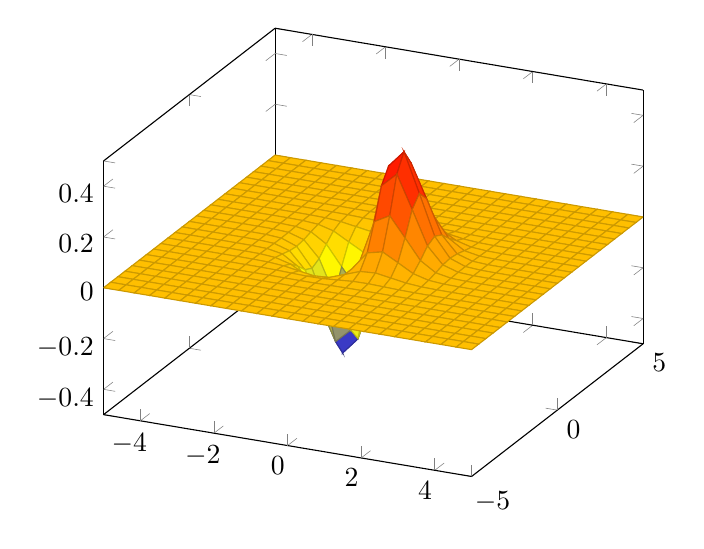
\begin{tikzpicture}
\begin{axis}
\addplot3[
    surf,
]
{exp(-x^2-y^2)*x};
\end{axis}
\end{tikzpicture}



1,$$a^2+b^2=c^2 \eqno (1)$$
2,\begin{equation} x^n+y^n=z^n \end{equation}abc
3,basing on($1$)
4,
\begin{equation}
\begin{array}{l}
a+b=1 \\
c+d=2
\end{array}
\end{equation}
5,split
\begin{equation}
\begin{split}
a+b=1\\
c+d=2
\end{split}
\end{equation}
split
\begin{equation}
\begin{split}
&a+b+c+d+r+f+s+w+d+r+f+d=\\
&c+d=2
\end{split}
\end{equation}
align,
\begin{align}
a+b = 1 \\
c+d = 2
\end{align}
align,notag,
\begin{align}
a+b = 1 \notag \\
c+d = 2
\end{align}
gather
\begin{gather}
a+b=1 \\
c+d=2
\end{gather}
multline,
\begin{multline}
a+b=1 \\
c+d=2
\end{multline}

cases

\begin{equation}
r=\begin{cases}
    \dfrac{r_{P}(x,y)}{r_{P}({x}',{y}')}, & \mbox{if } r_{P}\geq 0 \\
    \dfrac{r_{P}(x,y)}{r_{P}({z}',{y}')}, & \mbox{otherwise}.
  \end{cases}
\end{equation}

\[r=\begin{cases}
      \frac{r_{P}(x,y)}{r_{P}({x}',{y}')}, & \mbox{if } x<0 \\
      \frac{r_{P}(x,y)}{r_{P}({z}',{y}')}, & \mbox{otherwise}.
    \end{cases}\]
    

array

\[r=\{ \begin{array}{cc}
      \frac{r_{P}(x,y)}{r_{P}({x}',{y}')} & x<0 \\
      \frac{r_{P}(x,y)}{r_{P}({z}',{y}')} & otherwise
    \end{array}\]
    

split

\[\begin{split}
   a+b&=1 \\
   a+b&=2
\end{split}\]


aligned

\begin{equation}
  r= \begin{aligned}
      \frac{r_{P}(x,y)}{r_{P}({x}',{y}')} & x<0 \\
      \frac{r_{P}(x,y)}{r_{P}({z}',{y}')} & otherwise
    \end{aligned}
\end{equation}


[],
\[ a+b=1 \\ c+d=2 \]

$$ x(i) $$
$$ x_{(i)} $$

Given \eqref{equ:def1} \eqref{equ:def1}

abc\cite{IEEEhowto:IEEEtranpage,IEEEexample:shellCTANpage,IEEEexample:IEEEwebsite}

\subsection{subsection A}
subsection A
\begin{enumerate}
    \item enumerate enumerate enumerate enumerate enumerate enumerate enumerate enumerate enumerate enumerate

        enumerate
    \item enumerate enumerate enumerate enumerate enumerate enumerate enumerate  enumerate
\end{enumerate}

\begin{enumerate}[itemindent=2em]
    \item enumerate enumerate enumerate enumerate enumerate enumerate enumerate enumerate enumerate enumerate
    \item enumerate enumerate enumerate enumerate enumerate enumerate enumerate  enumerate
\end{enumerate}

\subsection{B}
    \emph{1) LM1:}subsection subsection subsection subsection subsection subsection subsection subsection subsection
\begin{enumerate}[itemindent=2em]
    \item enumerate enumerate enumerate enumerate enumerate enumerate enumerate enumerate enumerate enumerate
    \item enumerate enumerate enumerate enumerate enumerate enumerate enumerate  enumerate
\end{enumerate}

\subsection{c}
\begin{enumerate}[itemindent=2em]
    \item enumerate enumerate enumerate enumerate enumerate enumerate enumerate enumerate enumerate enumerate
    \item enumerate enumerate enumerate enumerate enumerate enumerate enumerate  enumerate
\end{enumerate}

\begin{center}
  center
\end{center}

\begin{itemize}
  \item itemize itemize itemize itemize itemize itemize itemize itemize itemize itemize itemize itemize itemize
  \item itemize
\end{itemize}

\begin{table}
  \centering
  table
  \caption{a}\label{a}
\end{table}

\bibliographystyle{IEEEtran}
\bibliography{IEEEabrv,IEEEexample}


\end{document}
